%----------------------------------------------------------------------------------------
%	PACKAGES AND DOCUMENT CONFIGURATIONS
%----------------------------------------------------------------------------------------

\documentclass{article}

\usepackage[brazilian]{babel}
\usepackage[utf8]{inputenc}
\usepackage[T1]{fontenc}
\usepackage{graphicx} % Required for the inclusion of images
\usepackage[a4paper, margin=4cm]{geometry}
\usepackage{url}
\usepackage{indentfirst}

\setlength{\parindent}{4em}
\setlength{\parskip}{0.5em}

%\setlength\parindent{0pt} % Removes all indentation from paragraphs

%----------------------------------------------------------------------------------------
%	DOCUMENT INFORMATION
%----------------------------------------------------------------------------------------

\title{Um Modelo Matemático para Batalhas de Exércitos de Cavalheiros} % Title

\author{Thales Luis Rodrigues Sabino} % Author name

\date{\today} % Date for the report

\begin{document}

\maketitle % Insert the title, author and date

\begin{center}
Relatório técnico do trabalho realizado na disciplina \textit{Instrução a Modelagem Matemática (2015-3)} do \textbf{Programa de Pós-Graduação em Modelagem Computacional (PGMC)} \textbf{da Universidade Federal de Juiz de Fora (UFJF)}.
\end{center}


\begin{center}
\textbf{Professor:} Rodrigo Weber dos Santos
\end{center}

% If you wish to include an abstract, uncomment the lines below
\begin{abstract}
Abstract text
\end{abstract}

%----------------------------------------------------------------------------------------
%	SECTION 1
%----------------------------------------------------------------------------------------

\section{Introdução}

Descoberta no século 19 na antiga Suméria, a cidade-estado de Lagash possui ruínas que contém registros que mostram vários aspectos da guerra travada com uma cidade-estado vizinha conhecida como Umma. Nas ruínas foram encontradas representações de soldados sendo devorados por abutres. A relíquia, hoje, encontra-se exposta no Museu do Louvre, em Paris \cite{firstwar}.

Fica claro que conflitos, armados ou não, sempre fizeram parte da história da humanidade. O orçamento dedicado a defesa de vários países corresponde a uma parte significativa do PIB gerado, tornando o aspecto bélico de extrema importância para a defesa e segurança de um país (procurar referência).

É evidente que uma parte significa do dinheiro investido nas forças militares é dedicada ao estudo de situações de combate, estratégias e maneiras eficientes de vencer as batalhas. O termo eficiente, nesse contexto, significa derrotar o inimigo sofrendo um número mínimo de baixas. 

Não faz parte do escopo deste trabalho a realização de uma discussão sobre os aspectos positivos, negativos e impactos sociais causados por conflitos, somente uma análise de um modelo  matemático que tenta capturar os aspectos de um conflito armado entre dois exércitos homogêneos.

Esse tipo de modelo matemático foi inicialmente desenvolvido por Frederick W. Lanchester (1914) (Figura \ref{fig:fw-lanchester}), um engenheiro britânico que que desenvolveu a teoria dos combates baseado em conflitos aéreos da Primeira Guerra Mundial na tentativa de explicar porque a concentração de forças era útil em combates modernos. As \textit{leis} de Lanchester são ensinadas e usadas em todos os colégios militares do mundo.

\begin{figure}[ht]
	\centering
	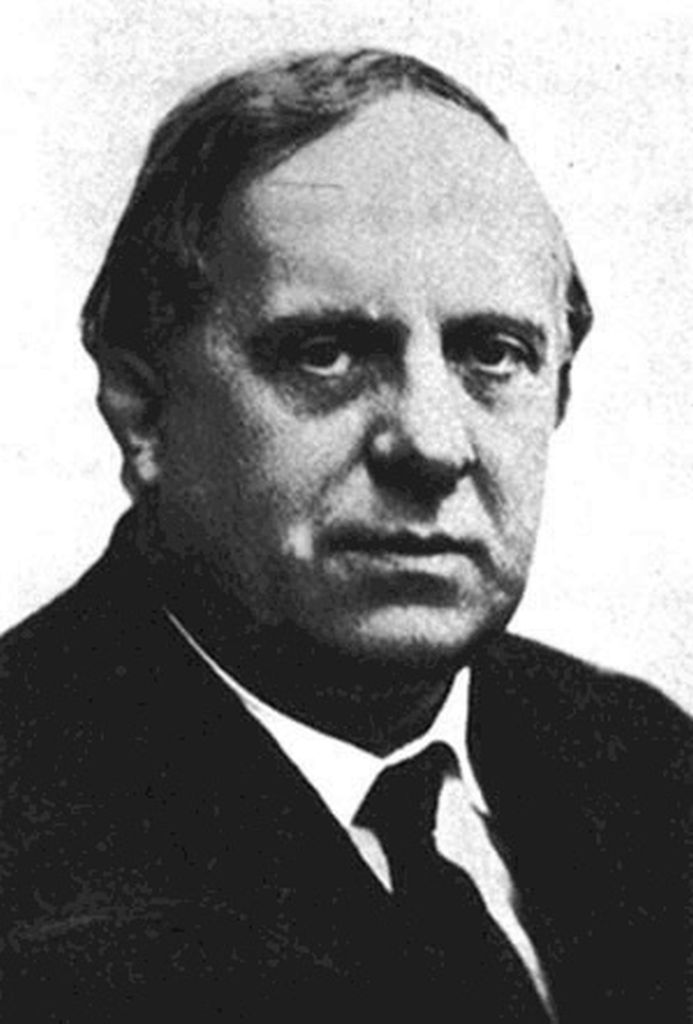
\includegraphics[width=0.3\linewidth]{figs/fw_lanchester_693x1024.jpg}
	\caption{Frederick Willian Lanchester}
	\label{fig:fw-lanchester}
\end{figure}

Existem dois tipos de modelos a serem considerados, \textbf{homogêneos} e \textbf{heterogêneos}. No modelo homogêneo, um único escalar é utilizado para representar o poder de combate de uma unidade e ambos os lados do conflito são considerados equivalentes quanto a eficiência em combate. O modelo homogêneo pode ser considerado de cunho \textit{acadêmico} e é aplicado na análise e revisão de \textit{batalhas históricos}, não sendo considerado um bom modelo para descrição de \textit{combates modernos}.

O objetivo deste trabalho é o desenvolvimento e análise de um modelo matemático capaz de representar o embate entre duas forças homogêneas, porém com munição disponível limitada. 

\section{Modelo Matemático}

\subsection{Dados de Entrada}

\section{Análise do Modelo}

%----------------------------------------------------------------------------------------
%	BIBLIOGRAPHY
%----------------------------------------------------------------------------------------

\bibliographystyle{acm}
\bibliography{references}

%----------------------------------------------------------------------------------------


\end{document}